
\de{ĐỀ THI HỌC KỲ II NĂM HỌC 2022-2023}{THPT Cầu Giấy - Hà Nội}
\begin{center}
	\textbf{PHẦN 1 - TRẮC NGHIỆM}
\end{center}
\Opensolutionfile{ans}[ans/ans]

%Câu 1...........................
\begin{ex}%[0X2Y3-1]%[Dự án đề kiểm tra HKII NH22-23- Thành Đức Trung]%[THPT Cầu Giấy - Hà Nội]
Viết khai triển theo công thức nhị thức Niu-tơn $\left(x-y\right)^5$.
\choice
{$x^5+5x^4 y+10x^3 y^2+10x^2 y^3+5xy^4+y^5$}
{$x^5+5x^4 y-10x^3 y^2-10x^2 y^3-5xy^4+y^5$}
{\True $x^5-5x^4 y+10x^3 y^2-10x^2 y^3+5xy^4-y^5$}
{$x^5+5x^4 y-10x^3 y^2+10x^2 y^3-5xy^4+y^5$}
\loigiai
{
Ta có $\left(x-y\right)^5=x^5-5x^4 y+10x^3 y^2-10x^2 y^3+5xy^4-y^5$.
}
\end{ex}

%Câu 2...........................
\begin{ex}%[0H4Y1-2]%[Dự án đề kiểm tra HKII NH22-23- Thành Đức Trung]%[THPT Cầu Giấy - Hà Nội]
Véc-tơ nào dưới đây là $1$ véc-tơ chỉ phương của đường thẳng song song với trục $Ox$?
\choice
{$\overrightarrow{u}=(1;-1)$}
{$\overrightarrow{u}=(0;1)$}
{$\overrightarrow{u}=(1;1)$}
{\True $\overrightarrow{u}=(1;0)$}
\loigiai
{
Trục $Ox$ có phương trình tổng quát là $y=0$, suy ra trục $Ox$ có $1$ véc-tơ chỉ phương là $(1;0)$. \\
Vậy đường thẳng song song với trục $Ox$ có $1$ véc-tơ chỉ phương là $\overrightarrow{u}=(1;0)$.
}
\end{ex}

%Câu 3...........................
\begin{ex}%[0X2B1-3]%[Dự án đề kiểm tra HKII NH22-23- Thành Đức Trung]%[THPT Cầu Giấy - Hà Nội]
Có bao nhiêu số chẵn mà mỗi số có $4$ chữ số đôi một khác nhau?
\choice
{\True $2296$}
{$2520$}
{$50000$}
{$4500$}
\loigiai
{
Gọi số cần lập là $\overline{abcd}$ với $a; b; c; d \in\{0; 1; 2; 3; 4; 5; 6; 7; 8; 9\}\left(a\ne0\right)$. \\
\textbf{Trường hợp 1.} Với $d=0$ suy ra $a$; $b$; $c$ có $\mathrm{A}_{9}^{3}$ cách chọn và sắp xếp. \\
\textbf{Trường hợp 2.} Với $d\in\{2;4;6;8\}$ suy ra $a$ có $8$ cách chọn, $b$ và $c$ có $\mathrm{A}_{8}^{2}$ cách chọn và sắp xếp. \\
Theo quy tắc nhân có $4\cdot8\cdot\mathrm{A}_{8}^{2} = 32\mathrm{A}_{8}^{2}$ số. \\
Vậy có $32\mathrm{A}_{8}^{2}+\mathrm{A}_{9}^{3}=2296$ số.
}
\end{ex}

%Câu 4...........................
\begin{ex}%[0H4G1-7]%[Dự án đề kiểm tra HKII NH22-23- Thành Đức Trung]%[THPT Cầu Giấy - Hà Nội]
Trong mặt phẳng $Oxy$, cho điểm $M(2;1)$. Đường thẳng $d$ đi qua $M$, cắt các tia $Ox$, $Oy$ lần lượt tại $A$ và $B$ ($A$, $B$ khác $O$) sao cho tam giác $OAB$ có diện tích nhỏ nhất. Phương trình đường thẳng $d$ là 
\choice
{$x-y-1=0$}
{$x-2y=0$}
{\True $x+2y-4=0$}
{$2x-y-3=0$}
\loigiai
{
Ta có $A$, $B$ là giao điểm của $d$ với hai tia $Ox$, $Oy$ nên gọi $A(a;0)$, $B(0;b)$ với ($a>0$ và $b>0$). \\
Phương trình $d$ theo đoạn chắn là $\dfrac{x}{a}+\dfrac{y}{b}=1$. \\
Do $M$ thuộc $d$ nên $\dfrac{2}{a}+\dfrac{1}{b}=1$. \hfill $(1)$ \\
Mặt khác $S_{\triangle OAB}=\dfrac{1}{2}\cdot OA\cdot OB=\dfrac{1}{2}|ab|=\dfrac{1}{2}ab$. \\
Để diện tích tam giác $OAB$ là nhỏ nhất thì $ab$ nhỏ nhất. \\
Ta có $1=\dfrac{2}{a}+\dfrac{1}{b}\geqslant2\sqrt{\dfrac{2}{ab}} \Leftrightarrow \dfrac{2}{ab}\leqslant\dfrac{1}{4} \Leftrightarrow ab\geqslant8$. \\
Dấu \lq\lq$=$\rq\rq\ xảy ra khi $\dfrac{2}{a}=\dfrac{1}{b}$. \hfill $(2)$ \\
Từ $(1)$ và $(2)$ ta có hệ $\heva{ & \dfrac{2}{a}+\dfrac{1}{b}=1 \\ & \dfrac{2}{a}=\dfrac{1}{b}} \Leftrightarrow \heva{ & \dfrac{2}{a}=\dfrac{1}{2} \\ & \dfrac{1}{b}=\dfrac{1}{2}} \Leftrightarrow \heva{ & a=4 \\ & b=2.}$ \\
Vậy phương trình $d$ là $\dfrac{x}{4}+\dfrac{y}{2} \Leftrightarrow x+2y-4=0$. 
}
\end{ex}

%Câu 5...........................
\begin{ex}%[0H3Y1-3]%[Dự án đề kiểm tra HKII NH22-23- Thành Đức Trung]%[THPT Cầu Giấy - Hà Nội]
Trong hệ trục tọa độ $Oxy$, cho hai điểm $M(1;1)$, $N(4;-1)$. Tính độ dài véc-tơ $\overrightarrow{MN}$.
\choice
{\True $\left|\overrightarrow{MN}\right|=\sqrt{13}$}
{$\left|\overrightarrow{MN}\right|=\sqrt{29}$}
{$\left|\overrightarrow{MN}\right|=5$}
{$\left|\overrightarrow{MN}\right|=3$}
\loigiai
{
Ta có $\overrightarrow{MN}=(3;-2) \Rightarrow \left|\overrightarrow{MN}\right|=\sqrt{3^2+\left(-2\right)^2}=\sqrt{13}$.
}
\end{ex}

%Câu 6...........................
\begin{ex}%[0H4Y2-1]%[Dự án đề kiểm tra HKII NH22-23- Thành Đức Trung]%[THPT Cầu Giấy - Hà Nội]
Tìm tọa độ tâm $I$ và bán kính $R$ của đường tròn $(C)\colon x^2+y^2-2x+4y+1=0$.
\choice
{$I(-1;2)$; $R=\sqrt{5}$}
{\True $I(1;-2)$; $R=2$}
{$I(1;-2)$; $R=4$}
{$I(-1;2)$; $R=4$}
\loigiai
{
Đường tròn $(C)$ có tâm $I(1;-2)$ và bán kính $R=\sqrt{1^2+\left(-2\right)^2-1}=2$.
}
\end{ex}

%Câu 7...........................
\begin{ex}%[0H4B2-3]%[Dự án đề kiểm tra HKII NH22-23- Thành Đức Trung]%[THPT Cầu Giấy - Hà Nội]
Đường tròn nào sau đây tiếp xúc với trục $Ox$?
\choice
{$x^2+y^2-5=0$}
{$x^2+y^2-10x-2y+1=0$}
{\True $x^2+y^2+6x+5y+9=0$}
{$x^2+y^2-10x=0$}
\loigiai
{
Phương trình trục $Ox$ là $y=0$. \\
Xét đường tròn $(C)\colon x^2+y^2+6x+5y+9=0$ có tâm $I\left(-3;-\dfrac{5}{2}\right)$ và bán kính $R=\dfrac{5}{2}$. \\
Ta có $\mathrm{d}(I,Ox)=\left|-\dfrac{5}{2}\right|=\dfrac{5}{2} \Rightarrow \mathrm{d}(I,Ox)=R$. \\
Vậy đường tròn $(C)\colon x^2+y^2+6x+5y+9=0$ tiếp xúc với trục $Ox$.
}
\end{ex}

%Câu 8...........................
\begin{ex}%[0X3K2-2]%[Dự án đề kiểm tra HKII NH22-23- Thành Đức Trung]%[THPT Cầu Giấy - Hà Nội]
Giải bóng chuyền cụm Thanh Xuân - Cầu Giấy gồm $9$ đội bóng tham dự, trong đó có $6$ đội trường ngoài và $3$ đội của trường THPT Cầu Giấy. Ban tổ chức cho bốc thăm ngẫu nhiên để chia thành $3$ bảng $A$, $B$, $C$ và mỗi bảng có $3$ đội. Tính xác suất để $3$ đội bóng của trường THPT Cầu Giấy ở $3$ bảng khác nhau.
\choice
{$\dfrac{3}{56}$}
{$\dfrac{53}{56}$}
{$\dfrac{19}{28}$}
{\True $\dfrac{9}{28}$}
\loigiai
{
Gọi $\Omega$ là không gian mẫu, suy ra $|\Omega|=\mathrm{C}_{9}^{3}\cdot\mathrm{C}_{6}^{3}\cdot\mathrm{C}_{3}^{3}=1680$. \\
Gọi $M$ là biến cố \lq\lq $3$ đội bóng của trường THPT Cầu Giấy ở $3$ bảng khác nhau\rq\rq.
\begin{itemize}
\item Chọn $1$ trong $3$ đội của trường Cầu Giấy và $2$ trong $6$ đội của trường ngoài có $\mathrm{C}_{3}^{1}\cdot\mathrm{C}_{6}^{2}=45$ cách.
\item Chọn $1$ trong $2$ đội còn lại của trường Cầu Giấy và $2$ trong $4$ đội còn lại của trường ngoài có $\mathrm{C}_{2}^{1}\cdot\mathrm{C}_{4}^{2}=12$ cách.
\item Đội còn lại của trường Cầu Giấy và $2$ đội còn lại của trường ngoài tạo thành $1$ bảng.
\end{itemize}
Suy ra $|M|=45\cdot12=540$ cách. \\
Vậy xác suất để $3$ đội bóng của trường THPT Cầu Giấy ở $3$ bảng khác nhau là
$$\mathrm{P}(A)=\dfrac{|M|}{|\Omega|}=\dfrac{540}{1680}=\dfrac{9}{28}.$$
}
\end{ex}

%Câu 9...........................
\begin{ex}%[0X2B3-2]%[Dự án đề kiểm tra HKII NH22-23- Thành Đức Trung]%[THPT Cầu Giấy - Hà Nội]
Tính tổng các hệ số trong khai triển nhị thức Niu-tơn của $\left(1-2x\right)^4$.
\choice
{$81$}
{$-81$}
{\True $1$}
{$-1$}
\loigiai
{
Tổng các hệ số trong khai triển nhị thức Niu-tơn là $\left(1-2\cdot1\right)^4=1$.
}
\end{ex}

%Câu 10...........................
\begin{ex}%[0X2Y2-1]%[Dự án đề kiểm tra HKII NH22-23- Thành Đức Trung]%[THPT Cầu Giấy - Hà Nội]
Có tất cả bao nhiêu cách xếp $6$ quyển sách khác nhau vào một hàng ngang trên giá sách?
\choice
{$6^6$}
{\True $6!$}
{$5!$}
{$6^5$}
\loigiai
{
Xếp $6$ quyển sách khác nhau vào một hàng ngang trên giá sách có $6!$ cách.
}
\end{ex}

%Câu 11...........................
\begin{ex}%[0X2B2-5]%[Dự án đề kiểm tra HKII NH22-23- Thành Đức Trung]%[THPT Cầu Giấy - Hà Nội]
Cho tập $A=\{0;1;2;3;4;5;6\}$. Từ tập $A$ có thể lập được bao nhiêu số tự nhiên gồm $5$ chữ số khác nhau và chia hết cho $5$.
\choice
{\True $660$}
{$679$}
{$523$}
{$432$}
\loigiai
{
Gọi số cần lập là $\overline{abcde}$. \\
\textbf{Trường hợp 1.} $e=0$, còn $6$ chữ số. \\
Chọn $4$ chữ số sắp xếp vào $4$ vị trí $a$; $b$; $c$; $d$ có $\mathrm{A}_{6}^{4}=360$. \\
Suy ra trường hợp 1 có $360$ số. \\
\textbf{Trường hợp 2.} $e=5$, còn $6$ chữ số. \\
Chọn $a$ trong $5$ chữ số $1$; $2$; $3$; $4$; $6$ có $5$ cách, còn $5$ chữ số.
Chọn $3$ chữ số sắp xếp vào $3$ vị trí $b$; $c$; $d$ có $\mathrm{A}_{5}^{3}=60$. \\
Suy ra trường hợp 2 có $5\cdot60=300$ số. \\
Vậy có $360+300=660$ số.
}
\end{ex}

%Câu 12...........................
\begin{ex}%[0X3B2-1]%[Dự án đề kiểm tra HKII NH22-23- Thành Đức Trung]%[THPT Cầu Giấy - Hà Nội]
Gieo một đồng tiền cân đối và đồng chất bốn lần. Xác suất để cả bốn lần xuất hiện mặt sấp là
\choice
{$\dfrac{2}{16}$}
{\True $\dfrac{1}{16}$}
{$\dfrac{6}{16}$}
{$\dfrac{4}{16}$}
\loigiai
{
Gieo một đồng tiền có $2$ khả năng. \\
Vậy xác suất để cả bốn lần xuất hiện mặt sấp là $\dfrac{1^4}{2^4}=\dfrac{1}{16}$.
}
\end{ex}

%Câu 13...........................
\begin{ex}%[0H4B1-2]%[Dự án đề kiểm tra HKII NH22-23- Thành Đức Trung]%[THPT Cầu Giấy - Hà Nội]
Trong mặt phẳng $Oxy$ cho điểm $M(1;2)$. Gọi $A$, $B$ là hình chiếu của $M$ lên $Ox$, $Oy$. Viết phương trình đường thẳng $AB$.
\choice
{$x+y-3=0$}
{\True $2x+y-2=0$}
{$x+2y-1=0$}
{$2x+y+2=0$}
\loigiai
{
Ta có $A(1;0)$ và $B(0;2)$. \\
Phương trình đường thẳng $AB$ là $\dfrac{x}{1}+\dfrac{y}{2}=1 \Leftrightarrow 2x+y-2=0$.
}
\end{ex}

%Câu 14...........................
\begin{ex}%[0X3B2-1]%[Dự án đề kiểm tra HKII NH22-23- Thành Đức Trung]%[THPT Cầu Giấy - Hà Nội]
Gieo một con súc sắc hai lần. Xác suất để ít nhất một lần xuất hiện mặt sáu chấm là
\choice
{$\dfrac{12}{36}$}
{$\dfrac{8}{36}$}
{\True $\dfrac{11}{36}$}
{$\dfrac{6}{36}$}
\loigiai
{
Gọi $\Omega$ là không gian mẫu, ta có $|\Omega|=6\cdot6=36$. \\
Gọi $A$ là biến cố \lq\lq ít nhất một lần xuất hiện mặt sáu chấm\rq\rq. \\
Suy ra $\overline{A}$ là biến cố \lq\lq cả hai lần không xuất hiện mặt sấu chấm\rq\rq. \\
Ta có $\left|\overline{A}\right|=5\cdot5=25$. \\
Vậy xác suất để ít nhất một lần xuất hiện mặt sáu chấm là là
$$\mathrm{P}(A)=1-\mathrm{P}\left(\overline{A}\right)=1-\dfrac{\left|\overline{A}\right|}{|\Omega|}=1-\dfrac{25}{36}=\dfrac{11}{36}.$$
}
\end{ex}

%Câu 15...........................
\begin{ex}%[0X1Y3-2]%[Dự án đề kiểm tra HKII NH22-23- Thành Đức Trung]%[THPT Cầu Giấy - Hà Nội]
Tiền lương hàng tháng của $7$ nhân viên trong một công ty du lịch lần lượt là $6{,}5$; $8{,}4$; $6{,}9$; $7{,}2$; $2{,}5$; $6{,}7$; $3{,}0$ (đơn vị: triệu đồng). Số trung vị của dãy số liệu thống kê trên bằng
\choice
{$7{,}2$ triệu đồng}
{$6{,}9$ triệu đồng}
{\True $6{,}7$ triệu đồng}
{$6{,}8$ triệu đồng}
\loigiai
{
Sắp xếp dãy số liệu theo thứ tự không giảm $2{,}5$; $3{,}0$; $6{,}5$; $6{,}7$; $6{,}9$; $7{,}2$; $8{,}4$. \\
Dãy số liệu có $7$ giá trị. \\
Vậy trung vị của dãy số liệu là $6{,}7$ triệu đồng.
}
\end{ex}

%Câu 16...........................
\begin{ex}%[0X1Y1-1]%[Dự án đề kiểm tra HKII NH22-23- Thành Đức Trung]%[THPT Cầu Giấy - Hà Nội]
Biết số gần đúng $a=3975421$ có độ chính xác $d=150$. Hãy ước lượng sai số tương đối của $a$.
\choice
{$\delta_a\leqslant0{,}0000039$}
{$\delta_a\leqslant0{,}0000099$}
{$\delta_a\geqslant0{,}0000039$}
{\True $\delta_a<0{,}000039$}
\loigiai
{
Sai số tương đối là $\delta_a\leqslant\dfrac{d}{|a|}=\dfrac{150}{3975421}\approx0{,}000037731$. \\
Vậy $\delta_a<0{,}000039$.
}
\end{ex}

%Câu 17...........................
\begin{ex}%[0X2B1-2]%[Dự án đề kiểm tra HKII NH22-23- Thành Đức Trung]%[THPT Cầu Giấy - Hà Nội]
Một hộp đựng $5$ bi đỏ và $4$ bi xanh. Có bao nhiêu cách lấy $2$ bi có đủ cả $2$ màu?
\choice
{$36$}
{$16$}
{\True $20$}
{$9$}
\loigiai
{
Lấy $1$ bi đỏ trong $5$ bi đỏ có $5$ cách. \\
Lấy $1$ bi xanh trong $4$ bi đỏ có $4$ cách. \\
Vậy có $5\cdot4=20$ cách lấy $2$ bi có đủ cả $2$ màu.
}
\end{ex}

%Câu 18...........................
\begin{ex}%[0H3B1-5]%[Dự án đề kiểm tra HKII NH22-23- Thành Đức Trung]%[THPT Cầu Giấy - Hà Nội]
Trong mặt phẳng tọa độ $Oxy$ cho $4$ điểm $A(1;-2), B(0;3), C(-3;4)$ và $D(-1;8)$. Phân tích $\overrightarrow{CD}$ qua $\overrightarrow{AB}$ và $\overrightarrow{AC}$.
\choice
{\True $\overrightarrow{CD}=2\overrightarrow{AB}-\overrightarrow{AC}$}
{$\overrightarrow{CD}=2\overrightarrow{AB}-\dfrac{1}{2}\overrightarrow{AC}$}
{$\overrightarrow{CD}=3\overrightarrow{AB}-\overrightarrow{AC}$}
{$\overrightarrow{CD}=2\overrightarrow{AB}-2\overrightarrow{AC}$}
\loigiai
{
Ta có $\heva{ & \overrightarrow{CD}=(2;4) \\ & \overrightarrow{AB}=(-1;5) \\ & \overrightarrow{AC}=(-4;6).}$ \\
Xét $\overrightarrow{CD}=m\overrightarrow{AB}+n\overrightarrow{AC} \Leftrightarrow \heva{ & 2=-m-4n \\ & 4=5m+6n} \Leftrightarrow \heva{ & m=2 \\ & n=-1.}$ \\
Vậy $\overrightarrow{CD}=2\overrightarrow{AB}-\overrightarrow{AC}$.
}
\end{ex}

%Câu 19...........................
\begin{ex}%[0H4B1-4]%[Dự án đề kiểm tra HKII NH22-23- Thành Đức Trung]%[THPT Cầu Giấy - Hà Nội]
Xác định tất cả các giá trị của $a$ để góc tạo bởi đường thẳng $\heva{ & x=9+at \\ & y=7-2t}$ $(t\in\mathbb{R})$ và đường thẳng $3x+4y-2=0$ bằng $45^{\circ}$.
\choice
{\True $a=\dfrac{2}{7}$, $a=-14$}
{$a=\dfrac{2}{7}$, $a=14$}
{$a=-2$, $a=-14$}
{$a=1$, $a=-14$}
\loigiai
{
Đường thẳng $d\colon \heva{ & x=9+at \\ & y=7-2t}$ có véc-tơ chỉ phương là $\overrightarrow{u}_{d}=(a;-2)$, suy ra véc-tơ pháp tuyến của $d$ là $\overrightarrow{n}_{d}=(2;a)$. \\
Đường thẳng $\Delta\colon 3x+4y-2=0$ có véc-tơ pháp tuyến là $\overrightarrow{n}_{\Delta}=(3;4)$. \\
Theo đề bài ta có
$$\begin{aligned}
& \ \cos 45^{\circ}=\dfrac{\left|\overrightarrow{n}_{d}\cdot\overrightarrow{n}_{\Delta}\right|}{\left|\overrightarrow{n}_{d}\right|\cdot\left|\overrightarrow{n}_{\Delta}\right|} \Leftrightarrow \dfrac{\sqrt{2}}{2}=\dfrac{|6+4a|}{\sqrt{4+a^2}\cdot5} \\
\Leftrightarrow & \ 5\sqrt{2a^2+8}=2|4a+6| \Leftrightarrow 25\left(2a^2+8\right)=4\left(4a+6\right)^2 \\
\Leftrightarrow & \ 14a^2+192a-56=0 \Leftrightarrow \hoac{ & a=\dfrac{2}{7} \\ & a=-14.}
\end{aligned}$$
}
\end{ex}

%Câu 20...........................
\begin{ex}%[0H4Y2-1]%[Dự án đề kiểm tra HKII NH22-23- Thành Đức Trung]%[THPT Cầu Giấy - Hà Nội]
Cho phương trình $x^2+y^2-2mx-4(m-2)y+6-m=0$ $(1)$. Điều kiện của $m$ để $(1)$ là phương trình của đường tròn.
\choice
{$m=2$}
{$\hoac{ & m=1 \\ & m=2}$}
{$1<m<2$}
{\True $\hoac{ & m<1 \\ & m>2}$}
\loigiai
{
Để $(1)$ là phương trình đường tròn thì
$$m^2+4\left(m-2\right)^2-6+m>0 \Leftrightarrow 5m^2-15m+10>0 \Leftrightarrow \hoac{ & m<1 \\ & m>2.}$$
}
\end{ex}

%Câu 21...........................
\begin{ex}%[0X1Y4-4]%[Dự án đề kiểm tra HKII NH22-23- Thành Đức Trung]%[THPT Cầu Giấy - Hà Nội]
Để đánh giá mức độ phân tán của các số liệu thống kê so với số trung bình, ta dùng đại lượng nào sau đây?
\choice
{Số trung bình}
{\True Phương sai}
{Mốt}
{Số trung vị}
\loigiai
{
Để đánh giá mức độ phân tán của các số liệu thống kê so với số trung bình, ta dùng đại lượng phương sai.
}
\end{ex}

%Câu 22...........................
\begin{ex}%[0H4B1-3]%[Dự án đề kiểm tra HKII NH22-23- Thành Đức Trung]%[THPT Cầu Giấy - Hà Nội]
Tìm các giá trị thực của tham số $m$ để đường thẳng $y=\left(m^2-3\right)x+3m+1$ song song với đường thẳng $y=x-5$.
\choice
{$\hoac{ & m=2 \\ & m=-2}$}
{$m=-2$}
{\True $m=2$}
{$\hoac{ & m=\sqrt{2} \\ & m=-\sqrt{2}}$}
\loigiai
{
Đường thẳng $y=\left(m^2-3\right)x+3m+1$ song song với đường thẳng $y=x-5$ khi
$$\heva{ & m^2-3=1 \\ & 3m+1\neq-5} \Leftrightarrow \heva{ & \hoac{ & m=2 \\ & m=-2} \\ & m\neq-2} \Leftrightarrow m=2.$$
}
\end{ex}

%Câu 23...........................
\begin{ex}%[0X1B1-4]%[Dự án đề kiểm tra HKII NH22-23- Thành Đức Trung]%[THPT Cầu Giấy - Hà Nội]
Theo thống kê, dân số Việt Nam năm $2022$ là $79715675$ người. Giả sử sai số tuyệt đối của số liệu thống kê này nhỏ hơn $10000$ người. Hãy viết số quy tròn của số trên.
\choice
{$79716000$ người}
{$79710000$ người}
{$79700000$ người}
{\True $79720000$ người}
\loigiai
{
Ta có $a=79715675$ và $\Delta_a<10000 \Rightarrow d=10000$. \\
Vậy số quy tròn của số $a$ là $79720000$.
}
\end{ex}

%Câu 24...........................
\begin{ex}%[0X1Y3-4]%[Dự án đề kiểm tra HKII NH22-23- Thành Đức Trung]%[THPT Cầu Giấy - Hà Nội]
Một tổ học sinh gồm $10$ học sinh có điểm kiểm tra cuối kì $1$ môn toán như sau $7$; $5$; $6$; $6$; $6$; $8$; $7$; $5$; $6$; $9$. Tìm mốt của dãy trên.
\choice
{$M_0=5$}
{\True $M_0=6$}
{$M_0=8$}
{$M_0=7$}
\loigiai
{
Sắp xếp lại dãy số liệu theo thứ tự không giảm $5$; $5$; $6$; $6$; $6$; $6$; $7$; $7$; $8$; $9$. \\
Mốt của dãy số liệu là $M_0=6$.
}
\end{ex}

%Câu 25...........................
\begin{ex}%[0X1B4-1]%[Dự án đề kiểm tra HKII NH22-23- Thành Đức Trung]%[THPT Cầu Giấy - Hà Nội]
Cho mẫu số liệu thống kê $\{1;2;3;4;5;6;7;8;9\}$. Tìm khoảng tứ phân vị của mẫu số liệu trên.
\choice
{$2$}
{$3$}
{$4$}
{\True $5$}
\loigiai
{
Ta có các tứ phân vị $Q_1=\dfrac{2+3}{2}=2{,}5$; $Q_2=5$ và $Q_3=\dfrac{7+8}{2}=7{,}5$. \\
Khoảng tứ phân vị là $\Delta_Q=Q_3-Q_1=5$.
}
\end{ex}


\Closesolutionfile{ans}
%\begin{center}
%	\textbf{ĐÁP ÁN}
%	\inputansbox{10}{ans/ans}	
%\end{center}
\begin{center}
	\textbf{PHẦN 2 - TỰ LUẬN}
\end{center}

%Câu 1...........................
\begin{bt}%[0X2B3-2]%[Dự án đề kiểm tra HKII NH22-23- Thành Đức Trung]%[THPT Cầu Giấy - Hà Nội]
Cho $\left(1-\dfrac{1}{2}x\right)^5 = a_0+a_1x+a_2x^2+a_3x^3+a_4x^4+a_5x^5$. Tính $a_3$.
\loigiai
{Ta có 
\begin{align*}
\left(1-\dfrac{1}{2}x\right)^5 &= \mathrm{C}_5^0 1^5 + \mathrm{C}_5^1 1^4 \left(-\dfrac{1}{2}x\right)+ \mathrm{C}_5^2 1^3 \left(-\dfrac{1}{2}x\right)^2+ \mathrm{C}_5^3 1^2 \left(-\dfrac{1}{2}x\right)^3+ \mathrm{C}_5^4 1 \left(-\dfrac{1}{2}x\right)^4+ \mathrm{C}_5^5 \left(-\dfrac{1}{2}x\right)^5\\&= 1-\dfrac{5}{2}x+\dfrac{5}{2}x^2-\dfrac{5}{4}x^3+\dfrac{5}{16}x^4-\dfrac{1}{32}x^5.
\end{align*}
Vậy $a_3=-\dfrac{5}{4}$.
}
\end{bt}

%Câu 2...........................
\begin{bt}%[0X1B4-3] %[Dự án đề kiểm tra HKII NH22-23- Thành Đức Trung]%[THPT Cầu Giấy - Hà Nội]
Biểu đồ đoạn thẳng ở hình bên biểu diễn tốc độ tăng trưởng GDP của Việt Nam giai đoạn $2012-2019$. Viết mẫu số liệu thống kê tốc độ tăng trưởng GDP nhận được từ biểu đồ ở hình bên. Tính số trung bình, phương sai và độ lệch chuẩn của mẫu số liệu đó.
\begin{center}
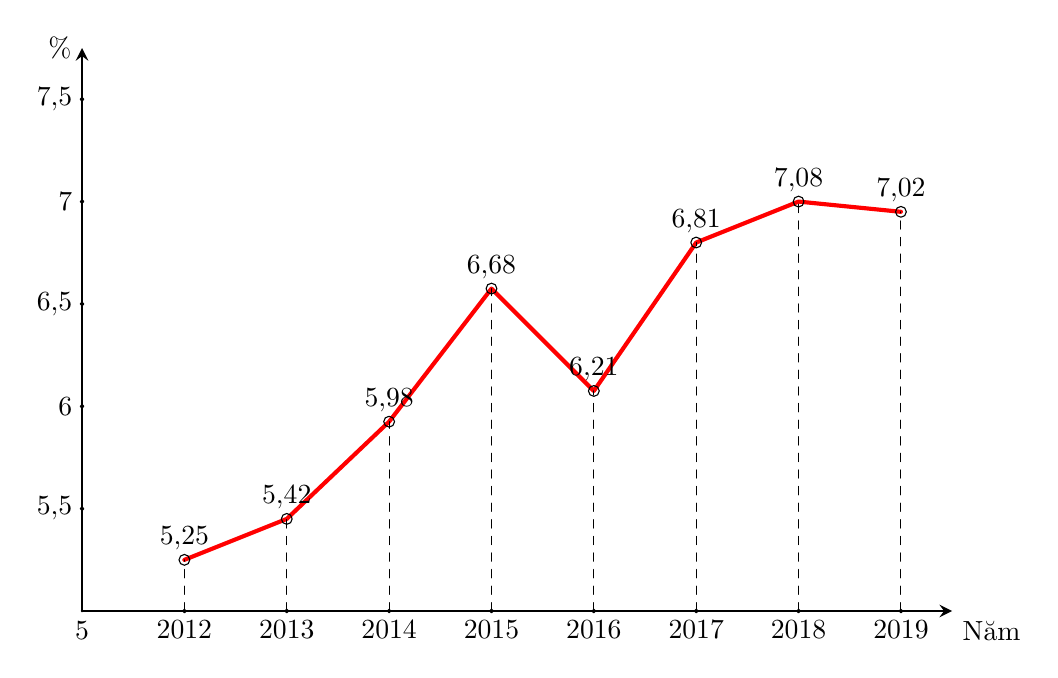
\begin{tikzpicture}[>=stealth,scale=0.65, line join = round, line cap = round]
\def\xmin{-1} \def\xmax{19}
\def\ymin{-1} \def\ymax{12} 
\draw[->,line width = 1pt] (0,0)--(17,0) node[below right]{Năm};
\draw[->,line width = 1pt] (0,0)node[below]{$5$} --(0,11) node[left]{$\%$};
\draw (2,0) node[below]{$2012$} circle (1pt);
\draw (4,0) node[below]{$2013$} circle (1pt);
\draw (6,0) node[below]{$2014$} circle (1pt);
\draw (8,0) node[below]{$2015$} circle (1pt);
\draw (10,0) node[below]{$2016$} circle (1pt);
\draw (12,0) node[below]{$2017$} circle (1pt);
\draw (14,0) node[below]{$2018$} circle (1pt);
\draw (16,0) node[below]{$2019$} circle (1pt);
\draw (0,2) node[left]{$5{,}5$} circle (1pt);
\draw (0,4) node[left]{$6$} circle (1pt);
\draw (0,6) node[left]{$6{,}5$} circle (1pt);
\draw (0,8) node[left]{$7$} circle (1pt);
\draw (0,10) node[left]{$7{,}5$} circle (1pt);
\draw [line width = 1.5pt,color=red] (2,1)--(4,1.8)--(6,3.7)--(8,6.3)--(10,4.3)--(12,7.2)--(14,8)--(16,7.8);
\draw [dashed] (2,0)--(2,1) (4,0)--(4,1.8) (6,0)--(6,3.7) (8,0)--(8,6.3) (10,0)--(10,4.3) (12,0)--(12,7.2) (14,0)--(14,8) (16,0)--(16,7.8);
\draw (2,1) node[above]{$5{,}25$} circle (3pt);
\draw (4,1.8) node[above]{$5{,}42$} circle (3pt);
\draw (6,3.7) node[above]{$5{,}98$} circle (3pt);
\draw (8,6.3) node[above]{$6{,}68$} circle (3pt);
\draw (10,4.3) node[above]{$6{,}21$} circle (3pt);
\draw (12,7.2) node[above]{$6{,}81$} circle (3pt);
\draw (14,8) node[above]{$7{,}08$} circle (3pt);
\draw (16,7.8) node[above]{$7{,}02$} circle (3pt);
\end{tikzpicture}
\end{center}
\loigiai
{
Sắp xếp mẫu số liệu trên $5{,}25\qquad 5{,}42\qquad 5{,}98\qquad 6{,}68\qquad 6{,}21\qquad 6{,}81\qquad 7{,}08 \qquad 7{,}02$.\\
Số trung bình của mẫu số liệu trên là
$$\overline{x}=\dfrac{5{,}25+ 5{,}42+ 5{,}98+ 6{,}68+ 6{,}21+ 6{,}81+ 7{,}08 + 7{,}02}{8}=6{,}30625\approx 6{,}31.$$
Phương sai của mẫu số liệu trên là
$$s^2=\dfrac{(5{,}25-6{,}31)^2+(5{,}42-6{,}31)^2+ \ldots + (7{,}02-6{,}31)^2}{8}=0{,}4398125.$$
Độ lệch chuẩn của mẫu số liệu trên là $s = \sqrt{s^2}\approx 0{,}66$.
}
\end{bt}

%Câu 3...........................
\begin{bt}%[0X3B2-3]%[Dự án đề kiểm tra HKII NH22-23- Thành Đức Trung]%[THPT Cầu Giấy - Hà Nội]
Trong một buổi khiêu vũ có đúng 10 cặp vợ chồng. Chọn ngẫu nhiên 2 người lên khiêu vũ đầu tiên. Xác suất của biến cố \lq\lq Chọn được 2 người là vợ chồng \rq\rq bằng bao nhiêu?
\loigiai
{
Gọi A là biến cố \lq\lq Chọn được 2 người là vợ chồng \rq\rq.\\
Số cách chọn ngẫu nhiên 2 người lên khiêu vũ từ nhóm gồm 20 người là
\[n\left(\Omega\right) = \mathrm{C}_{20}^2 = 190.\]
Chọn ra 1 cặp vợ chồng trong tổng số 10 cặp vợ chồng là
\[n\left(\mathrm{A}\right) = \mathrm{C}_{10}^1 = 10.\]
Vậy có 10 kết quả thuận lợi cho biến cố A. Suy ra xác suất của biến cố A là
\[\mathrm{P}(\mathrm{A}) = \frac{n\left(\mathrm{A}\right)}{n\left(\Omega\right)} = \frac{10}{190} = \frac{1}{19}.\]
}
\end{bt}

%Câu 4...........................
\begin{bt}%[0H4K1-4]%[Dự án đề kiểm tra HKII NH22-23- Thành Đức Trung]%[THPT Cầu Giấy - Hà Nội]
\begin{enumerate}
\item Cho đường thẳng $d\colon3x-2y+1=0$ và $M(1;2)$. Viết phương trình đường thẳng $\Delta$ đi qua $M$ và tạo với $d$ một góc $45^\circ$.
\item Lập phương trình đường tròn $(C)$ có tâm $I(1;-1)$ và có một tiếp tuyến là $\Delta\colon5x-12y-1=0$.
\end{enumerate}
\loigiai
{\begin{enumerate}
\item Gọi $\overrightarrow{n}(a;b)$ với $(a^2+b^2>0)$ là véc-tơ pháp tuyến của đường thẳng $\Delta$.
Vì $\Delta$ tạo với $d$ một góc $45^\circ$ nên 
\begin{align*}
&\cos 45^\circ = \dfrac{|3a-2b|}{\sqrt{3^2+(-2)^2}\cdot\sqrt{a^2+b^2}}\\\Leftrightarrow& \dfrac{\sqrt{26}}{2}\sqrt{a^2+b^2}=|3a-2b|\\\Leftrightarrow&\dfrac{5}{2}a^2-\dfrac{5}{2}b^2-12ab =0\\\Leftrightarrow&\hoac{&a=-\dfrac{1}{5}b\\&a = 5b.}
\end{align*}
Với $a=-\dfrac{1}{5}b$, chọn $b =-5\Rightarrow a = 1$, suy ra $\Delta\colon 1(x-1)-5(y-2)=0\Leftrightarrow x-5y+9=0$.\\
Với $a=5b$, chọn $b =1\Rightarrow a = 5$, suy ra $\Delta\colon 5(x-1)+1(y-2)=0\Leftrightarrow 5x+y-7=0$.\\
\item Vì $\Delta$ là tiếp tuyến của $(C)$ nên $
R = \mathrm{d}(I, \Delta)\Leftrightarrow R = \dfrac{|1\cdot5+1\cdot12-1|}{\sqrt{5^2+(-12)^2}}=\dfrac{16}{13}$.\\
Phương trình đường tròn tâm $I$ có tiếp tuyến là $\Delta$ có dạng $(x-1)^2+(y+1)^2=\left(\dfrac{16}{13}\right)^2$.
\end{enumerate}
}
\end{bt}

%Câu 5...........................
\begin{bt}%[0H3K2-7]%[Dự án đề kiểm tra HKII NH22-23- Thành Đức Trung]%[THPT Cầu Giấy - Hà Nội]
%\immini
%{
Một vật đồng thời bị ba lực tác động: lực tác động thứ nhất $\overrightarrow{F}_1$ có độ lớn là $1500 \mathrm{~N}$, lực tác động thứ hai $\overrightarrow{F_2}$ có độ lớn là $600 \mathrm{~N}$, lực tác động thứ ba $F_3$ có độ lớn là $800 \mathrm{~N}$. Các lực này được biểu diễn bằng những vectơ như hình 2 , với $\left(\overrightarrow{F_1}, \overrightarrow{F_2}\right)=30^\circ$; $\left(\overrightarrow{F_1}, \overrightarrow{F_3}\right)=45^\circ$; $\left(\overrightarrow{F_2}, \overrightarrow{F_3}\right)=75^\circ$. Tính độ lớn lực tổng hợp tác động lên vật (làm tròn kết quả đến hàng đơn vị).
\begin{center}
\definecolor{battleshipgrey}{rgb}{0.52, 0.52, 0.51}
\begin{tikzpicture}[line join=round, line cap=round,scale=1,transform shape]
\clip (-5,-4) rectangle (5,4);
\tikzset{t/.pic={
\def\M{ 
(-3.3,2.2)--(-3.2,2.2)--(-3.2,1.25)--(-3.3,1.25)--cycle
(-3.2,2.15)--(-3,2.15)--(-3,1.2)--(-3.2,1.2)--cycle
(-3.2,2)--(-3,2)
(-3.2,1.85)--(-3,1.85)
(-3.2,1.7)--(-3,1.7)
(-3.2,1.55)--(-3,1.55)
(-3.2,1.38)--(-3,1.38)
;
}
\fill[white] \M;
\draw[line width=.25mm]\M;
}}
\tikzset{h/.pic={
\def\N{ 
(-3.7,2.6)
..controls +(0:.6) and +(90:.1) ..(-3.3,1.3)--(-3.2,1.25)
..controls +(-90:.8) and +(90:1.5) ..(-1.3,0)
..controls +(-90:1.5) and +(90:.8) ..(-3.2,-1.25)--(-3.3,-1.35)
..controls +(-90:.1) and +(0:.6) ..(-3.7,-2.6)--cycle
(-3.7,-2.8)--(-3.7,2.8)--(-4,2.8)--(-4,-2.8)--cycle
;
}
\fill[battleshipgrey] \N;
\draw\N;
}}
\path
(-2.18,0) coordinate (A)
(4,0) coordinate (B)
(.5,1.6) coordinate (C)
(.5,-2.5) coordinate (D)
;
\draw pic["$30^\circ$", draw=black, angle eccentricity=2, angle radius=.6cm]{angle=B--A--C};
\draw pic["$45^\circ$", draw=black, double, angle eccentricity=2, angle radius=.6cm]{angle=D--A--B};
\path
(0,0)pic[scale=1]{t}
(0,0)pic[scale=1,yscale=-1]{t}
(0,0)pic[scale=1]{h};
\draw[fill=white] (-2.18,0) circle (.32);
\draw[->] (-2.18,0)--(.5,1.6);
\draw[->] (-2.18,0)--(4,0);
\draw[->] (-2.18,0)--(.5,-2.5);
\node at (4,0) [above left]{$\overrightarrow{F}_1$};
\node at (.5,1.6) [above left]{$\overrightarrow{F}_2$};
\node at (.5,-2.5) [below left]{$\overrightarrow{F}_3$};
\end{tikzpicture}
\end{center}
%}
%{
%\begin{tikzpicture}[scale=.85, font=\footnotesize, >=stealth]  
%\draw[fill = black] (0,0) circle (10pt);
%\draw[fill = white] (0,0) circle (5pt);
%\path
%(0,0) coordinate (O)
%(6,0) coordinate (A)
%(3,2) coordinate (B)
%(3,-3) coordinate (C)
%;
%\draw[->,thick,red] (O) -- (A) node[right]{$\overrightarrow{F_1}$};
%\draw[->,thick,red] (O) -- (B) node[above right]{$\overrightarrow{F_2}$};
%\draw[->,thick,red] (O) -- (C) node[below right]{$\overrightarrow{F_3}$};
%\draw (1,0) node[above]{$30^\circ$};\draw (1,0) node[below]{$45^\circ$};
%\end{tikzpicture}
%}
\loigiai
{
\begin{center}
\begin{tikzpicture}[scale=1, font=\footnotesize, >=stealth]  
\draw[fill = black] (0,0) circle (10pt);
\draw[fill = white] (0,0) circle (5pt);
\path
(0,0) coordinate (O)
(6,0) coordinate (A)
(3,2) coordinate (B)
(3,-3) coordinate (C)
($(B)+(C)$) coordinate (G)
($(G)+(A)$) coordinate (H)
;
\draw[->,thick,red] (O) -- (A) node[above]{$\overrightarrow{F_1}$};
\draw[->,thick,red] (O) -- (B) node[above right]{$\overrightarrow{F_2}$};
\draw[->,thick,red] (O) -- (C) node[below right]{$\overrightarrow{F_3}$};
\draw[dashed,blue] (B)--(G)--(C);
\draw[dashed,green] (A)--(H)--(G);
\draw[->,thick,blue] (O) -- (G) node [below right]{$\overrightarrow{F_{23}}$};
\draw[->,thick,green] (O) -- (H) node [right] {$\overrightarrow{F}$};
\end{tikzpicture}
\end{center}
\begin{itemize}
\item $\overrightarrow{F}=\overrightarrow{F}_1+\overrightarrow{F_2}+\overrightarrow{F_3}=\overrightarrow{F_1}+\overrightarrow{F_{23}}$. \\
\item $\begin{aligned}[t]
& \overrightarrow{F_{23}}=\overrightarrow{F_2}+\overrightarrow{F_3} \\
 \Rightarrow & F_{23}^2=F_2^2+F_3^2+2F_2F_3\cos \left(\overrightarrow{F_2}, \overrightarrow{F_3}\right)=600^2+800^2+2\cdot600 \cdot 800 \cdot \cos 75^{\circ}	=1248466{,}283~(\mathrm{N}) \\
\Rightarrow & F_{23}=\sqrt{1248466{,}283}\approx 1117{,}35~(\mathrm{N}).
\end{aligned}$ \\
\item $\begin{aligned}[t]
& \cos \left(\overrightarrow{F_{23}}, \overrightarrow{F_3}\right)=\frac{F_{23}^2+F_3^2-F_2^2}{2 \cdot F_{23} \cdot F_3}=\frac{1248466,283+800^2-600^2}{2\cdot1117{,}35\cdot800} \approx 0{,}855. \\
\Rightarrow & \left(\overrightarrow{F_{23}}, \overrightarrow{F_3}\right) \approx 31^{\circ} \Rightarrow\left(\overrightarrow{F_{23}}, \overrightarrow{F_1}\right)=45^{\circ}-31^{\circ}=14^\circ.
\end{aligned}$ \\
\item $\begin{aligned}[t]
& \overrightarrow{F}=\overrightarrow{F}_1+\overrightarrow{F_{23}} \\
\Rightarrow & F^2\begin{aligned}[t]&=F_{23}^2+F_1^2+2 F_{23}F_1\cos \left(\overrightarrow{F_{23}}, \overrightarrow{F_1}\right) \\
&=1248466{,}283+1500^2+2\cdot1117{,}35\cdot1500 \cdot \cos 14^{\circ} \\
&=6750946{,}072.
\end{aligned} \\
\Rightarrow & F=\sqrt{6750946{,}072} \approx 2598~(\mathrm{N}).
\end{aligned}$
\end{itemize}
Vậy độ lớn của lực tổng hợp tác động lên vật bằng $2598$ Newton.
}
\end{bt}